\documentclass[10pt,twoside,slovak,a4paper]{article}

\usepackage[slovak]{babel}
\usepackage[IL2]{fontenc}
\usepackage[utf8]{inputenc}
\usepackage{graphicx}
\usepackage{url}
\usepackage{hyperref}
\usepackage{cite}




\pagestyle{headings}

\title{Rolling updates\thanks{Semestrálny projekt v predmete Metódy inžinierskej práce, ak. rok 2021/22, vedenie: Ján Lučansky}}

\author{Silvia Kuchtová\\[2pt]
	{\small Slovenská technická univerzita v Bratislave}\\
	{\small Fakulta informatiky a informačných technológií}\\
	{\small \texttt{xkuchtovas@stuba.sk}}
	}

\date{\small 18. december 2021} 



\begin{document}
\maketitle

\begin{abstract}
Priebežná aktualizácia je široko používaná technika na aktualizáciu softvéru, pričom služba poskytovaná viacerými inštanciami softvéru zostáva dostupná. Aktualizácie softvéru v  systémoch, a najmä v rozsiahlych systémoch webových služieb sú nevyhnutné a ich ich množstvo sa zvyšuje.  Keď 
aktualizácia zlyhá, následky môžu byť vážne. Je to dokonca ťažšie, keď chceme zachovať dostupnosť a obsluhu systému zákazníkom počas aktualizácie. Problémy s takýmto dynamickými aktualizáciami softvéru sú dobre známe. V súčasnosti je bežnou praxou používanie priebežných aktualizácií, keď je služba poskytovaná viacerými inštanciami softvéru. V jednom okamihu sa pri priebežnej aktualizácii odstráni malý počet inštancií, ktoré používajú starú verziu softvéru a nahradí ich inštanciami v novej verzii. Tento proces sa opakuje, až kým nie sú všetky inštancie v starej verzii nahradené.

\end{abstract}

\section{Úvod}

Tento článok vám pomôže lepšie pochopiť, čo sú to prebežné aktualizácie (rolling updates) a ako v skratke tieto aktualizácie fungujú. Tieto základné informácie si objasníme v častiac ~\ref{1}  a  ~\ref{2}  . V článku si spomenieme aj výhody a nevýhody, ktoré takéto aktualizácie prinášajú a v nakoniec to celé zhodnotíme v záverečnej časti ~\ref{3}.

\section{Čo sú priebežné aktualizácie}\label{1}

Väčšina programov sa časom aktualizuje, zvyčajne prostredníctvom štandardného vydania aktualizácie. Pri štandardných aktualizáciách vývojár softvéru vytvorí úplne novú verziu programu a aktualizácie sa bežne objavujú každých niekoľko týždňov alebo mesiacov. Ak vývojár používa schému priebežného vydávania, postupuje sa inak. Namiesto zriedkavých aktualizácií sa aktualizácie bežne vykonávajú každý deň alebo každých niekoľko dní. Vývojár tiež pracuje len na aktualizácii jednej programovej vetvy, zatiaľ čo štandardné aktualizácie pracujú na viacerých vetvách.\\
\textbf{Priebežné aktualizovanie} je preto postup pri aktualizácii softvéru, ktorý namiesto vytvárania veľkých aktualizácií naraz zahŕňa mnoho priebežných aktualizácií.  Výhodou tejto metódy je, že aktualizácie vychádzajú oveľa rýchlejšie a zvyčajne sa s nimi programátorom ľahšie pracuje. Zároveň však aktualizácie nemusia byť také dôkladné\cite{web2}.

\section{Ako priebežné aktualizácie fungujú}\label{2}
Pri tradičnej aktualizácii softvéru sa aplikačné servery odstavia, kým sa ich softvér aktualizuje a testuje, a potom sa opäť uvedú do prevádzky. To môže mať za následok značné prestoje aplikácie - najmä ak neočakávané chyby alebo problémy prinútia vývojára vrátiť inštaláciu na predchádzajúcu verziu.\\\\
Pri priebežnej aktualizácii je v danom čase mimo prevádzky len časť kapacity servera pre aplikáciu. Príkladom môže byť trojvrstvová aplikácia pozostávajúca z front end, back end a databázy,  s tromi uzlami v každej vrstve. Každý z troch uzlov front-end aplikačného servera prijíma prevádzku cez \textbf{load balancer} \textit{ (vyrovnávač záťaže)}. Pri tradičnej aktualizácii vyrovnávač záťaže uzavrie všetku prevádzku aplikácie, aby servery prešli do režimu offline a aktualizovali sa. Pri priebežnom nasadení môže organizácia vyradiť jeden z uzlov v každej vrstve z prevádzky, pričom vyrovnávač záťaže je nakonfigurovaný tak, aby presmeroval prevádzku na zostávajúce servery, na ktorých stále beží overená, aktuálna verzia softvéru. Nečinné servery prijímajú aktualizácie a testujú sa; zostávajúce servery v režime online podporujú prevádzku používateľov\cite{web1} .\\\\

\begin{figure}[htbp]
  \centering
  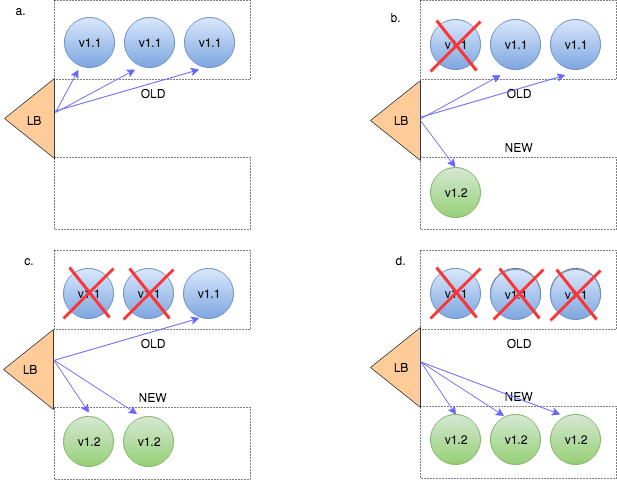
\includegraphics[width=8cm]{RampedDep1.png}
  \caption{Schéma postupu priebežných aktualizácií.}
  \label{4}
  \cite{picture}
\end{figure}

Skrátene povedané, pri priebežnej aktualizácii sa odstráni malý počet inštancií starej verzie a potom ich nahradí inštanciami novej verzie. Tento proces sa opakuje, až kým sú všetky inštancie starej verzie nahradené\cite{7034783}. Tento postup môžme vidieť aj na predchádzajúsom obrázku~\ref{4} \\\\
Priebežné aktualizácie môžu zahŕňať \underline{testovaciu fázu}, v ktorej vyrovnávač záťaže smeruje len obmedzenú alebo testovaciu prevádzku, kým sa nový softvér nakonfiguruje a vyskúša. To nemá vplyv na  používateľov, ktorí stále pristupujú k aplikácii na zostávajúcich serveroch, ktoré ešte neboli aktualizované\cite{web1}. \\\\
Po úspešnom otestovaní softvéru sa server vráti do prevádzky a ďalší uzol servera sa odpojí, aby sa proces zopakoval, pričom sa pokračuje, kým nie sú všetky uzly servera v klastri aktualizované a beží na nich požadovaná verzia softvéru aplikácie. \textbf{Celá aplikácia bola nepretržite dostupná počas celého postupného aktualizovania.}\cite{web1}

\section{Výhody a nevýhody}
	Jednou z hlavných výhod priebežného vydávania pre vývojára je, že zvyčajne môže aktualizácie vytvárať v malom časovom úseku. Aktualizovaný program bude tiež často fungovať lepšie. Program je neustále aktualizovaný, takže by mal zaznamenať vyššiu rýchlosť aplikácie a chyby by mali byť rýchlo odstránené.\\\\
Ďalšou výhodou priebežných nasadení je, že ich možno ľahko vrátiť späť, ak sa niečo pokazí. Ak v priebehu aktualizácie zaznamenáme problémy - zvyčajne je možné "vrátiť" postupné nasadenie a začať odstraňovať novú verziu aplikácie a znovu spustiť starú verziu.\\\\
	Hoci má priebežné vydávanie programu svoje výhody, má aj niektoré nevýhody. Pri štandardných aktualizáciách má vývojár dostatok času na diagnostikovanie prípadných chýb alebo závažných problémov ovplyvňujúcich program. V schéme priebežných aktualizácií vývojár neustále vykonáva aktualizácie, takže si nemusí všimnúť závažné problémy. Je tiež menej času na testovanie aktualizácií, takže sa môžu vyskytnúť zjavné chyby, ktoré by sa pri štandardných aktualizáciách opravili. Program sa mení tak často, že aj keď sú zmeny malé, robia softvér zraniteľným voči vírusom a hackerským problémom.\\\\
	 Počas vykonávania priebežnej aktualizácie bude prostredie trochu nepredvídateľné, pretože v ňom súčasne bežia rôzne verzie aplikácie. A napokon, vyradenie serverov z prevádzky znamená, že počas aktualizácie je k dispozícii menšia kapacita pre prevádzku používateľov.\\\\
V rozsiahlych systémoch a aplikáciách je zapojených veľa inštancií, a preto priebežná aktualizácia trvá hodiny alebo aj oveľa dlhšie. Počas dlhej priebežnej aktualizácie sú zlyhania a v skutočnom dátovom centre môže obnova po poruche a údržba systému trvať hodiny alebo dni. \cite{7586059}


\section{Blue/green model}
Blue/green deployment je model vydania aplikácie, ktorý postupne prenáša používateľskú prevádzku z predchádzajúcej verzie aplikácie  na takmer identickú novú verziu. \\\\
Stará verzia sa môže nazývať modré prostredie, zatiaľ čo nová verzia sa môže označovať ako zelené prostredie. Po úplnom prenose produkčnej prevádzky z modrého do zeleného prostredia môže byť modré prostredie v pohotovostnom režime pre prípad vrátenia alebo stiahnutia z produkcie a aktualizácie, aby sa stalo šablónou, na základe ktorej sa vykoná ďalšia aktualizácia.


\section{Záver}\label{3}
V tomto článku sme predstavili priebežné aktualizácie, funkciu, ktorá je užitočná, pretože umožňuje aktualizovať bežiace aplikácie na novšie  bez prerušenia prevádzky. Tento model však má svoje nedostatky, z ktorch by pár mohlo byť v budúcnosti odstránených. Zamedzenm chýb by mohlo byť aj zavedenie dlhšej testovacej fázy alebo vykonávanie aktualizácií v dlhšom časovom úseky, pre lepšiu kontrolu chybovosti novej verzie. 

\bibliographystyle{plain}
\bibliography{zdroje}


\end{document}

